% Session E technical-report draft. Suggested compiler: XeLaTeX.
% XeLaTeX build and rendered-page QA are recorded in checkpoint.json.
% Snapshot: 2026-10-07. Forty-four cells / 10752 request executions; 340 jointly eligible commits (292 Host, 48 Recompute).
\documentclass[UTF8,fontset=fandol,a4paper,10pt]{ctexart}
\usepackage[margin=2cm]{geometry}
\usepackage{amsmath,amssymb,booktabs,tabularx,array}
\usepackage[hidelinks]{hyperref}
\usepackage{xurl}
\usepackage{enumitem}
\usepackage{xcolor}
\usepackage{graphicx}
\graphicspath{{E_restore_choice_20261004/figures/}{figures/}}
\hypersetup{pdftitle={固定调度机制下被抢占请求的原生恢复方式选择：技术报告初稿}}
\setlist{nosep,leftmargin=1.6em}
\setlength{\parindent}{2em}
\setlength{\parskip}{2pt}
\newcommand{\code}[1]{\nolinkurl{#1}}
\newcommand{\pending}[1]{\textcolor{red!65!black}{\textbf{[待回填：#1]}}}
\title{固定调度机制下被抢占请求的原生恢复方式选择\\
\large 阶段报告：真实恢复域、服务代价与测量边界}
\author{独立研究会话 E}
\date{2026 年 10 月 7 日}

\begin{document}
\maketitle
\begin{abstract}
在支持 Host KV 卸载的推理服务中，被抢占请求再次获得恢复机会时，可以加载已有合法 KV，或利用原生重算重建状态。本文固定恢复目标选择机制、victim、队列、服务量子和准入，仅改变恢复执行方式。现已完成四十四格、10752 次请求执行，包含 340 次两路径共同可行的原生提交，其中 292 次 Host、48 次重算。正常容量三档 QA 的八格均无恢复；自然长摘要在 72.1015625 GiB GPU KV 预算下实际执行了两条原生路径。两组各四格的单次恢复干预均通过目标前历史与调度一致性检查。E249 的 Host 下一输出为 139--141 ms，重算为 157--158 ms，并令邻请求延后约 87 ms。E223 的 Host 恢复后再次被抢占，下一输出约 1.02 s；改为重算后降至 161--162 ms，却将再次抢占转移给邻请求，使其下一输出延后约 0.80 s。两个事件的动作排名不同，但前缀与命中覆盖也不同，不能归为状态的增量解释力。跨动作改变后续内容与工作量，完整服务时间不是等工作量加速证据。独立 MultiNews 六臂的输出与调度完全一致，但均无恢复；27 个新闻组的 ROUGE-L 宏均值为 27.243，固定人工核验仍发现事实错误。后续八臂验证了原生剩余调度 token 预算规则，但它与固定长度阈值的实际动作、原生调度轨迹及输出完全一致，故已从活动实现中淘汰。新完成的容量余量六臂产生了超出长度阈值的实际动作差异：同一短请求的完整 56-token 输出由 Host 的 68--70 s 提前至 22--27 s 完成，但再次抢占转移给邻请求，跨策略工作量改变且同策略计时漂移明显。随后固定 Host 的 GPU 遥测开关四臂保持完全相同的输出与原生调度，但关闭后尾段仍有 7.813 s 漂移，开关效应变号。本文仍未建立质量合格服务或状态感知规则的全局收益；320 请求独立新闻容量域候选尚未运行。
\end{abstract}

\section{问题与可检验范围}
\label{sec:problem}
设请求 $r$ 在时刻 $t$ 已收到的输入为 $P_r$，已经对外产生的 token 为 $Y_r^{\le t}$。恢复必须保留的已知历史为
\begin{equation}
 H_r(t)=P_r\Vert Y_r^{\le t},\qquad n_r(t)=|H_r(t)|.
\end{equation}
选择器只读取当前和历史观测，不能使用未来输出长度，也不能先执行两条路径再选择较快结果。本文考虑如下两个动作：
\begin{itemize}
 \item $a=\mathrm{Host}$：加载 Host 中已经就绪、与当前历史一致的原生 KV 前缀，并由原生路径补齐未命中的必要尾部。
 \item $a=\mathrm{Recompute}$：保留同一个请求及其已知 token 历史，经原生调度器和模型执行器重建必要 KV，随后继续生成。
\end{itemize}
Host 命中并不要求覆盖全部历史；两条路径最终都必须到达原请求下一次合法生成所需的完整状态。研究对象不是重新提交一个新请求，也不是把已经生成的文本当作新的回答重新采样。

第一版固定恢复目标、抢占对象选择、FCFS 队列、token 预算、准入检查和传输实现。动作导致后续系统状态自然变化是实验结果的一部分；不能为了强行对齐两臂的执行轨迹，再修改调度器。对照固定的是外部到达序列、资源预算和机制参数，而不是要求两次运行具有完全相同的抢占事件集合。

待检验假设是：孤立恢复速度可能没有反映传输排队、GPU 计算竞争及其他请求的停顿。不过，这只是实验动机；本文不预设存在交叉点，不预设状态感知规则优于最佳固定动作。若当前运行域始终由一个动作占优，或只有一条路径可合法执行，应直接报告该边界。

\section{成本口径与正确性边界}
\label{sec:cost}
令 $t_r^{\mathrm{next}}$ 为一次已提交恢复选择之后该请求首次新输出的时间。局部观测为
\begin{equation}
 L_r^{\mathrm{next}}=t_r^{\mathrm{next}}-t_r^{\mathrm{decision}}.
\end{equation}
该时间包含真实排队、传输、重算和调度等待，不能用孤立复制时间替代。若请求在下一次输出前再次被抢占，多次选择可能对应同一次输出；分析器保留这种关联，不将这些记录当作独立因果样本。

全局观测使用所有请求的外部到达 $A_i$、完成 $C_i$ 以及连续输出时间 $O_{i,k}$，至少报告平均完成时延、整体完工时间以及生成间隔：
\begin{equation}
 \overline F=\frac{1}{N}\sum_{i=1}^N(C_i-A_i),\quad
 M=\max_i C_i-\min_i A_i,\quad
 G_{i,k}=O_{i,k}-O_{i,k-1}\;(k>1).
\end{equation}
同时报告 TTFT、每请求最大停顿、间隔分位数和未完成请求。正常容量主组保留自然 EOS，预先声明的输出上限只限定合法生成范围；必须同时报告实际输出长度、EOS/长度截断数量和输出差异，不能假设各臂工作量恒等。固定输出只用于另行标记的等工作量诊断。自然停止本身也不构成任务质量或生产 goodput 证据。

\paragraph{已经发生的 STORE 是沉没成本。}
在 $t$ 之前，为请求保存 KV 的计算与传输已经真实发生。无论随后选择哪个动作，该历史成本都保留在整段服务统计中；比较当前动作的增量影响时，不能将其再次计入 Host 分支，也不能将其记作重算节省。两臂均保留同一原生 STORE 机制。动作以后新增的计算、LOAD、STORE 和排队仍由真实执行统计。异步传输与计算可能重叠，CUDA 事件时间可用于诊断，却不能简单相加来重建端到端墙钟时间。

\paragraph{完整状态容量。}
设每个 GPU KV block 容纳 $b$ 个 token，当前已知历史至少需要
\begin{equation}
 B_r=\left\lceil n_r(t)/b\right\rceil.
\end{equation}
当前薄适配器仅在 $B_r+B_{\mathrm{reserved}}+B_{\mathrm{watermark}}\le B_{\mathrm{free}}$ 时允许改变原生结果，并继续执行原生分配器的全部检查。运行器打开完整序列容量约束。该条件不是声称只加载较短 Host 前缀便可减少完整状态所需容量，也不替代模型执行的其他内存要求。

\paragraph{请求连续性。}
选择前后核对对象身份、全部已知 token、采样参数对象、输出进度、状态及停止原因，记录前缀哈希。输出必须单调扩展已有序列，重建未完成时不得冒出新的输出 token。首轮使用 greedy 路径；不据此宣称已经验证随机采样的 RNG 状态等价。前三档 QA 正式测量未执行恢复动作；后续摘要组的 46 次共同可行提交通过已知历史、对象状态和输出连续性检查，但这仍不是 KV 逐元素、logits 或随机采样等价验证。即使历史完全相同，批形状改变也可能引入数值差异，故跨臂 token 差异应如实保留，并在后续自然任务中单独评估质量。

\section{原生接口与薄适配}
\label{sec:implementation}
实现依据本地保存的 vLLM 0.26.0 源码快照。原生 connector scheduler 的
\code{get_num_new_matched_tokens} 返回可用外部前缀；随后
\code{update_state_after_alloc} 在 GPU 分配后准备加载，并调用
\code{manager.prepare_load}。原生主调度器的
\code{_preempt_request} 重置已计算进度，请求对象仍持有
\code{all_token_ids}，供调度器恢复计算。源文件路径和哈希由项目的
\code{native_sources/} 与 \code{source_manifest.json} 保存。

\code{selector.py} 在原生 lookup 之后作一次小范围适配。只有已经抢占过、存在正的就绪 Host 命中且满足共同容量条件的请求进入可选集合。Host 策略原样保留命中；Recompute 策略将 connector 的命中元数据同步归零并返回 \code{(0, False)}，让同一个原生请求进入正常计算路径。选择器不分配另一套 KV，不实现新的重算执行器，也不在选择前执行传输或模型计算。双方都经过原生 lookup，保留其共同的查找行为。

lookup 可能被尝试多次而未真正获得资源，因此尝试次数不等于执行决策数。当前记录以
\code{update_state_after_alloc} 为提交边界，分别保存偏好、返回结果与实际外部 token 数。尚在等待本请求原生传输时沿用原生延期；Host 未命中时沿用原生重算；共同容量不足时保留原生结果与准入检查。这些 fallback 独立计数，不作为选择器成功样本隐藏。

适配依赖私有字段，故版本变化可能破坏假设。运行时限定原生 CPU offloading、单 KV group、非滑窗及关闭 APC，并检查预热后缓存重置、实际 GPU/Host 存储字节数和 Host pinned 属性。断言失败应留下失败记录并停止该实验格。已完成 GPU 服务的配置包括固定 Host、固定 Recompute、显式长度阈值及剩余调度预算规则。后者在八臂真实服务中通过预算核验，却未产生超出固定阈值的动作信息，已从活动实现移除；当前 H/R/L 原生分支保持不变，容量余量规则已完成下文的六臂原生验证。完整预算实现与 22 项 CPU 测试保存在\code{execution/source_snapshots/oct07_budget_r01/}，供复现已完成实验。前三档 QA 的八格正式服务动作全部为零；摘要组的实际两路径执行记录见第~\ref{sec:summaryresults} 节。执行证据与历史连续性检查不等于完整数值正确性验证。共同固定输出预热的选择器关闭，不能将其中 LOAD 补算为正式事件。

\section{首轮实验协议}
\label{sec:protocol}
表~\ref{tab:config} 给出已完成三档正常容量实验的统一协议，结果见第~\ref{sec:results} 节。GPU KV 采用 \code{gpu_memory_utilization=0.9} 下的原生 profiling，不设置显式 KV 字节上限；记录实际可用 block 数和张量存储字节数。每组只初始化并 profile 一个引擎，各臂复用该引擎；组间重新初始化并分别核对实际容量，不以相同 utilization 参数代替容量证据。本文主结果不包含显式限容实验。
\begin{table}[ht]
\centering\small
\caption{正常容量首轮配置；最终以每组日志及资源断言为准。}
\label{tab:config}
\begin{tabularx}{\linewidth}{@{}p{0.23\linewidth}X@{}}
\toprule
项目 & 配置 \\
\midrule
设备与模型 & RTX PRO 6000 Blackwell Server Edition；服务器已有 OLMoE 本地快照 \\
软件与执行 & vLLM 0.26.0；PyTorch 2.11.0；Transformers 5.17.0；BF16、eager、原生 Triton MoE \\
KV 预算 & GPU 原生 0.9 profiling；pinned Host 32 GiB；记录 chunk 舍入后实际容量；APC、推测解码关闭 \\
调度与准入 & FCFS；最多 256 请求；每步 2048 token；完整当前历史必须可容纳 \\
工作负载 & 64、192、256 请求三档；固定 1 短:3 长；相同档位各臂输入和外部到达相同，外部到达均为 0 \\
输入与输出上限 & 短 GSM8K 输入 661--约 800 token、输出上限 256；长完整 QA 输入 2699--3271 token、输出上限 512 \\
生成与顺序 & greedy、自然 EOS，256/512 为上限；低负载和接近容量候选各 Host/Recompute 两臂，高压力候选用 Host/Recompute/Recompute/Host \\
引擎与隔离 & 同组各臂复用同一引擎；每臂前相同完整预热和缓存重置；组间释放 GPU \\
\bottomrule
\end{tabularx}
\end{table}

三组使用同一已核验 GPU，设备 UUID、软件版本与运行时源文件哈希随原始结果保存；汇总器的配置指纹本身不替代源码哈希核验。

工作负载由 \code{inputs_pro6000/freeze_receipt.json} 在 CPU 侧冻结。短提示来自公开 GSM8K test 的 64 个选定样本及既有八示例前缀~\cite{gsm8k}；长提示来自 LongBench \code{multifieldqa_en} 的 17 条完整自然 QA~\cite{longbench}，包含原上下文和问题，不通过截断或重复拼接文本构成长输入。长任务循环复用这些样本，但每次提交是独立请求并使用独立缓存身份；关闭 APC，不能借重复提示获得 GPU 前缀复用。三档分别含 33、65、81 个不同提示，是重复自然请求的压力探针，不能作为独立任务泛化或质量结论。

\begin{table}[ht]
\centering\small
\caption{冻结的三档负载。容量列仅是假设所有请求同时驻留且均生成到上限时的完整 KV 上界估计，非实测分配或抢占证据。}
\label{tab:loads}
\begin{tabular}{@{}lrrrr@{}}
\toprule
候选档位 & 请求数 & 短/长请求 & 不同提示数 & 上界估计 (GiB) \\
\midrule
低负载 & 64 & 16/48 & 33 & 22.35 \\
接近容量 & 192 & 48/144 & 65 & 67.23 \\
高压力 & 256 & 64/192 & 81 & 89.66 \\
\bottomrule
\end{tabular}
\end{table}

表~\ref{tab:loads} 的估计按 16-token block 舍入，来自冻结清单；实际驻留时间、原生准入与完成顺序可能使峰值占用显著低于此值。“接近容量”和“高压力”是候选负载标签，须由实际 block 使用、队列、抢占与合法 Host 命中记录确认。Host 预算也不保证恢复命中，原生驻留和淘汰决定可用前缀。

同组每臂开始前，先排空上一 episode 的原生传输并重置 Host/GPU 缓存；再关闭选择器，用该档全部请求执行相同原生 Host 预热，排空 STORE/LOAD 后再次重置。当前共同预热仍忽略 EOS 并生成到各自上限，用于覆盖并发批形状；这些输出不属于正式测量。复位后正式主组使用自然 EOS，不能把预热期间的抢占当作主组恢复。检查请求队列、connector 作业与缓存空闲基线，防止前臂状态泄漏。计时从重置后的正式 episode 开始；版本、配置、输入清单、预热成本、资源、状态和原始事件均单独落盘。若预热成本需要缩减，应依据运行证据另行冻结相同的新预热方案，不在组内改动。不能事后删除不利运行；超时或断言失败时保留部分轨迹与失败原因。

每组持有共同 GPU 锁，初始化及各臂测量前后核对设备与计算进程，结束后释放 GPU。锁等待和初始化不计入正式 episode；所有中止另行记录，不作为已完成测量格。

\code{run_cell.py} 记录外部到达与实际入队时间、每次原生调度的计算区间、抢占、选择/提交、每个新输出及完成时刻，以及原生 LOAD/STORE 报告。输出时刻取本地同步 \code{engine.step()} 返回后的观测，包含 Python 驱动与插桩开销，尚不是网络流式客户端时延。\code{analyze.py} 汇总上述局部与全局指标，并区分 lookup 尝试、提交和 fallback。所有统计以真实服务为基础，不离线扣除估计开销构造另一个动作。

低负载首先检验正常容量基线与追踪完整性；高压力 ABBA 再检查方向的反序稳定性。正常容量下没有抢占或没有两路径均合法的恢复事件也是有效结果，恢复时延应记为不适用，不能填零后宣传收益。一次突发和重复自然提示不足以支持稳定尾分位数或统计显著性论断。两臂的事件数可能不同；不得将跨运行、同长度但不同系统历史的恢复事件直接视为随机配对。可对照的是外部请求及整段服务，事件分组只作为解释性诊断。

\section{最小在线规则与后续推进条件}
\label{sec:future-rule}
若真实对照出现可重复且值得利用的差异，先增加长度/成本阈值
\begin{equation}
 \pi_{\ell}(n)=
 \begin{cases}\mathrm{Recompute},&n\le\tau,\\
 \mathrm{Host},&n>\tau,
 \end{cases}
\end{equation}
并在验证运行前冻结 $\tau$。成本阈值须独立校准，结构性长度阈值须说明由来。若测量不支持这一方向，应调整或弃用该假设，而不是强制制造阈值交叉。成本基线只比较未来的 LOAD/必要尾部计算与重建成本。

当前轨迹同时留有待处理 LOAD 数、队列规模和近期原生步骤时间，目的是诊断，不代表在线规则应同时使用所有特征。两组单事件干预各自匹配目标前历史，但两个目标之间的前缀与命中覆盖也不同；待处理 LOAD 很少非零，尚不能识别这些状态的增量价值。E249 的实际 token 预算耗尽与邻请求延后，为单信号验证提供了具体执行依据；第~\ref{sec:budget-next} 节报告已完成的剩余预算规则八臂实验及其淘汰结论。该规则不是由两个事件拟合的时延预测器，实测也没有超出长度阈值的动作信息。禁止使用未来输出长度，禁止将事后最优动作算作在线收益。

比较对象必须包含最佳固定方式、固定长度/成本阈值和增加一个状态信号的规则。若规则退化为固定阈值，应直接报告等价性；若状态在控制长度后没有增量解释力，应删除该状态模型。若局部恢复变快而全局完成或生成间隔恶化，下一步先检查该动作占用了哪些请求的执行机会，而不是继续扩大参数搜索。

信号稳定后再扩展到独立任务、不同到达形状与至少一个独立负载；报告任务质量、完整开销及所有失败。需要另行测量有无插桩的差异、选择器运行开销与随机采样连续性。主组 GSM8K 与长 QA 虽保留自然 EOS，17 条长 QA 的循环独立提交仍不增加不同任务数量，不能直接提供泛化或问答质量结论。\code{--fixed-output} 仅用于明确标记的等工作量诊断，不能用其强制生成的压力替代自然主组证据。

\section{相关工作与研究定位}
CacheOPT 按模型和硬件对长度建立重算、swap 成本函数，其比较包含 swap-out 和 swap-in；系统还联合改变其他 KV 分配和调度机制~\cite{cacheopt}。Stream2LLM 在 preemption 时采用硬件成本选择，其实现明确使用闲置系统静态 profile，并独立比较调度与驱逐策略~\cite{stream2llm}。这两者是成本基线来源；在本文 STORE 已支付的边界上必须重新标定。本次补充核对了 Stream2LLM 官方 commit \code{5e2763d} 的 v1 调度器与 engine core：前者在抢占时比较两个静态成本函数，后者对重算均值和 swap-in 加 swap-out 的均值分别拟合二次曲线。其函数自变量为当前分配调用的 \code{num_new_tokens}，不能未经核对就改述为 victim 前缀长度。本文尚未复现其整套系统；将其成本思想移至 STORE 已付的恢复边界，需要单独声明并重新校准。

UnboxKV 已实测并发、GPU KV 容量与模型影响 swap/recompute 排名，且指出重复 prefill 会影响调度~\cite{unboxkv}。因此，观察到负载相关排名变化本身不是本文可主张的新发现。Cake 双向并行计算前缀与加载后缀，并调整与其他请求共享算力的优先级~\cite{cake}；CacheGen 根据网络条件在不同压缩 KV 与文本重算之间适配~\cite{cachegen}。这些工作已经建立资源状态与计算/加载选择之间的关系，其混合执行、编码或调度变化超出本文第一版动作空间。

LUMEN 在故障恢复时根据 worker 负载，必要时放弃 checkpoint 本地性并改派请求重算~\cite{lumen}。其目的地选择与本文固定目的地的动作不同，但使“首次负载感知恢复”这一表述不成立。ShadowServe 研究 KV 解压与模型计算的干扰，说明局部数据路径指标不足以替代完整服务指标~\cite{shadowserve}；本文没有解压步骤，不能沿用其干扰量级。本文当前定位是一个受控问题与最小实现，是否具有超出强近邻的实证价值仍取决于后续真实数据。

\paragraph{静态成本对照的实际覆盖。}
对已完成预算组、E249 与 E223 组的 178 次合法提交作有界审查，共有 32 个已知长度/Host 命中长度 $(K,H)$ 点，仅 4 点有双动作观测；严格精确点查表只覆盖其中 52 次提交。下文容量余量组又实际覆盖了 $(719,704)$ 的 H/R，且对应前史一致，因此取消重复采集该点的计划。这些是有争用参考负载下的经验点，不能称为 idle profile，不能无声外推到其他命中覆盖，也不足以声称完整强近邻对照已完成。拟实施的对照仅适配 Stream2LLM 的静态选择思想，使用 STORE 已付后直到正确下一输出的原生完整剩余路径，保留未覆盖域；实现方案与覆盖证据见\code{strong_neighbor_plan.txt}及\code{calibration_coverage.txt}。

\section{正常容量 QA 结果与计时边界}
\label{sec:results}
\paragraph{八格真实服务完成。}
\code{execution/oct07_low_r02/}、\code{oct07_near_r02/} 和 \code{oct07_high_r01/} 分别保存 64、192、256 请求组。前两组各两臂，后一组为 ABBA，共八格、1536 次正式请求执行。各格均完成，无分析错误、失效或未完成格；输入、固定配置、实际资源及预热重置按组核对。独立原始轨迹复算保存在 \code{low64_results.txt}、\code{near192_results.txt} 和 \code{high256_results.txt}。这些是请求执行次数，不是 1536 个独立任务或统计重复。

\begin{table}[ht]
\centering\small
\caption{全部正式测量。H/R 仅表示所配置的 Host/Recompute 策略，数字表示组内顺序；八格实际恢复动作全部为零，表中差异不是恢复收益。}
\label{tab:mainresults}
\begin{tabular}{@{}llrrrrr@{}}
\toprule
请求数 & 臂 & 输出 tokens & 完工 (s) & 均值 (s) & P95 (s) & P99 间隔 (ms) \\
\midrule
64  & H0 & 8,694  & 9.693  & 3.957  & 7.541  & 35.726 \\
64  & R1 & 8,694  & 9.583  & 3.979  & 7.567  & 35.480 \\
192 & H0 & 28,648 & 19.548 & 9.966  & 17.783 & 48.592 \\
192 & R1 & 28,648 & 25.769 & 11.160 & 23.529 & 58.165 \\
256 & H0 & 37,730 & 27.289 & 12.298 & 22.757 & 59.638 \\
256 & R1 & 37,730 & 22.945 & 11.478 & 20.948 & 51.881 \\
256 & R2 & 37,730 & 22.872 & 11.455 & 20.906 & 51.856 \\
256 & H3 & 37,730 & 22.927 & 11.499 & 20.970 & 52.474 \\
\bottomrule
\end{tabular}
\end{table}

表~\ref{tab:mainresults} 的均值及 P95 均为从固定外部到达计算的完成时延，生成间隔不含 TTFT。各档的逐请求 greedy 输出序列跨臂全同，完成/停止元数据也相同；256 档的六个两两比较均为 256/256 一致。每臂以长度上限结束的请求数在三档分别为 3、14、20，其余自然停止。输出 cap 之和分别为 28,672、86,016、114,688，显著大于实际输出，不能以 cap 代替工作量。该一致性检查既不是任务质量评分，也不能验证尚未执行的恢复状态不变量。

\paragraph{合法恢复域仍为空。}
三组独立初始化所得实际 GPU KV 均为 72.1015625 GiB、36,916 blocks，pinned Host 均为 32 GiB、16,384 blocks。八格的抢占请求数、恢复尝试、Host-ready 事件、共同可行事件、已提交动作和 fallback 均为零，LOAD 字节与传输数也均为零。因此 decision-to-next-output 没有样本，应记为不适用，而不是零时延。表~\ref{tab:capacityresults} 给出实际观测；“接近容量”和“高压力”候选标签均未在正式自然输出下形成恢复竞争。

\begin{table}[ht]
\centering\small
\caption{各档正式测量的实际峰值及每臂 STORE；同档各臂相同。GPU 峰值取 schedule/step/preempt 边界，含初始常占的 1 block；Host 峰值取 step 边界。}
\label{tab:capacityresults}
\begin{tabular}{@{}lrrrr@{}}
\toprule
请求数 & GPU 使用 blocks & GPU 占比 & Host blocks & STORE (GiB) \\
\midrule
64  & 7,545  & 20.4383\% & 10,137 & 19.798828 \\
192 & 15,892 & 43.0491\% & 16,384 & 59.876953 \\
256 & 17,881 & 48.4370\% & 16,384 & 79.804688 \\
\bottomrule
\end{tabular}
\end{table}

这些占用不是完整 allocator 高水位或物理 GPU 总显存占比。Host 常驻满额也不意味着发生恢复：192/256 档持续 STORE 与原生淘汰可以发生在零 LOAD 的服务过程中。最早进入的自然任务可在后续 prefill 建立 KV 前完成，因而增加外部请求数不必然增加同时驻留到上限的状态；这是一种与结果相容的解释，尚不能单独确认为全部容量变化的原因。

\paragraph{完整保留 STORE。}
三档每臂 STORE 字节数分别为 21,258,829,824、64,292,388,864、85,689,630,720，已报告传输数分别为 685、2214、2924。按表~\ref{tab:mainresults} 的臂顺序，CUDA-event 持续时间和分别为 64 档 0.410424/0.413987 s，192 档 1.264007/1.302383 s，256 档 1.692707/1.673955/1.678274/1.685173 s。统计保留整个正式 episode 及 drain，不含共同预热与初始化，未从重算配置扣除已支付 STORE。192/256 档不仅总字节相同，每批 STORE 的字节和尺寸序列也相同。事件时间可以重叠，不是关键路径等待；不能用其与墙钟作简单加减来排除传输排队的间接影响。包含空 LOAD 字段的元数据报告数不等于 LOAD 次数。

\paragraph{自然退休与实际驻留。}
在三档首次达到观测 KV 峰值时，已有 14、94、145 个请求完成，全部为自然停止；已开始但未完成的请求仅为 50、98、109 个。256 请求组的峰值可分解为 145 个已完成、106 个已输出未完成、3 个正在 prefill 及 2 个尚未开始的请求。长 QA 的平均实际输出仅为 153.1、165.1、162.9 token。轨迹支持自然退休限制同时驻留的解释，但不证明容量已经平台化：192 到 256 时峰值仍增加 5.39 个百分点。新摘要任务只检验更长自然输出是否改变该边界，不保证出现恢复。详细计数见 \code{capacity_retirement_note.txt}。

\paragraph{同工作量下的零动作漂移。}
按外部请求身份规范化内部随机 ID 后，192 档全部 728 步、256 档全部 784 步在各自组内完全相同：包括 scheduled 请求顺序、计算位置区间、token 数、已知/已生成进度和 schedule 后空闲 block。两档原生调度 token 数分别为 491,770 和 655,437；运行/等待队列大小、GPU 空闲量、待处理 LOAD 数和 Host 常驻量也逐步一致。于是观察到的时间差不能解释为选择器改变了这些工作。

192 档 R1 比 H0 多 6.220755 s（31.8\%）；256 档首末同为 Host 的 H0/H3 相差 4.361749 s（19.0\%），而其余三臂完工时间仅相差 0.072711 s。漂移跟随不同运行位置，不能由 ABBA 按策略平均转化为收益。两档约 89\%/90\% 的 step 时间差在 schedule 记录与 step 返回之间，该区间仍混有主机派发、GPU 执行/等待和输出处理。端点未见其他 GPU 进程，cgroup 未记限额/OOM；这些检查不能排除测量中的 CPU 争用、时钟变化或异步等待。详细逐步诊断保存在上述结果文件，目前只定位了持续慢步，未确定根因。

\paragraph{预热与正式恢复必须分开。}
256 档四次共同预热各生成固定 114,688 tokens、执行 1057 步，GPU 最小空闲 block 为零，日志确有原生 LOAD；正式测量仅生成 37,730 tokens，峰值占用 48.44\%，且无恢复。预热期间 \code{selector.enabled=False}，空抢占列表表示没有记录，不能推断预热零抢占，也不能将其 LOAD 补算成正式选择器覆盖。四次预热完成时间为 56.839/56.326/57.711/61.539 s，规范化调度相同；最后一次预热较慢而其正式测量较快，不能用简单的“后运行更热”解释全部漂移。192/256 组可见的 JIT warning 均在首臂预热，未发现正式测量中的数秒单步尖峰；这不排除未记录开销，但不支持将持续漂移直接归于该次编译。

\paragraph{前三档的证据边界。}
这三档 QA 单独验证了服务链、原始追踪、共同资源/预热复位和零恢复下的输出一致性，以及 192/256 档逐步调度的一致性。其恢复指标无样本；零动作时延漂移也不构成方法收益。下一节报告追加长输出探针后实际激活的恢复事件，仍分别保留连续性、性能与任务质量的验证边界。

\section{正常容量自然长摘要：两条路径已真实执行}
\label{sec:summaryresults}
\paragraph{负载与完成状态。}
三档 QA 都没有恢复后，追加一个预先冻结的自然长输出探针，见\code{natural_pressure_next.txt}。256 请求保持 64 条原 GSM8K，另 192 条请求使用三篇原始完整文档，每篇独立请求 64 次，要求 600--750 词的详细摘要；三个 prompt 分别为 3052、2871、2736 tokens，输出 cap 为 1024。没有截断、拼接或填充输入；仍为自然 EOS、\code{min_tokens=0}。四臂保持正常 GPU 0.9 profiling、Host 32 GiB 及原有全部机制，在同一引擎执行 H/R/R/H，每臂使用相同预热与重置。

\code{execution/oct07_summary_r01/} 的四臂全部完成，共 1024 次请求执行，实际 GPU KV 容量与前述三档相同，观测峰值均达到 100\%。四臂各有 36 次原生抢占和 36 次恢复提交。H0/H3 各有 14 次共同可行 Host 提交及 22 次 Host 未命中原生重算 fallback；R1/R2 各有 9 次共同可行重算及 27 次相同类型 fallback。共同可行提交合计 46 次，其中 42 次已有生成历史。选择器尝试次数不等于提交次数：H0 有 605 次 lookup 尝试，其中 517 次共同容量不足尝试均未提交。不能将这些重试充作可选恢复样本。

\begin{table}[ht]
\centering\small
\caption{自然摘要四臂实测。R1 的回传干扰明确保留；恢复均值对应各臂自身的合法提交集合，跨策略不构成配对动作效应。}
\label{tab:summaryresults}
\begin{tabular}{@{}lrrrrr@{}}
\toprule
臂 & 输出 tokens & 完工(s) & 平均完成(s) & 最大停顿(s) & 合法恢复均值(s) \\
\midrule
H0 & 189,436 & 111.590 & 63.607 & 48.237 & 0.3594 \\
R1（有干扰） & 191,080 & 100.438 & 65.655 & 55.856 & 0.1813 \\
R2 & 191,080 & 116.308 & 68.502 & 55.123 & 0.1813 \\
H3 & 189,436 & 114.128 & 65.848 & 49.650 & 0.3228 \\
\bottomrule
\end{tabular}
\end{table}

\paragraph{局部等待不是全服务收益。}
合法提交到下一次输出的重算均值较小，但两个策略的恢复请求、历史与命中覆盖并不相同，不能据此称重算快了某个百分比。Host 可只命中已知历史的一部分，例如 3266 个已知 token 只命中 768，或 3539 只命中 1040；后续必要尾部仍须真实计算。H0 有两个提交关联同一次后续输出，反映恢复后再被抢占；14 个事件不是 14 个独立试验。H0 的抢占到提交平均等待约 18.215 s、最长约 48.051 s，远大于提交后的平均等待。因此必须保留表中的全请求完成与生成停顿，不能用局部恢复均值替代服务收益。

\paragraph{实际传输与重建工作。}
每个 Host 臂执行 4,349,493,248 bytes LOAD、14 次传输，CUDA-event 时间和为 0.080246/0.079025 s；两重算臂 LOAD 为零。每个 Host 臂 STORE 为 103,551,074,304 bytes，每个重算臂为 103,309,901,824 bytes；全部保留，没有减去历史 STORE 构造收益。Host/重算每臂实际调度 860,683/894,640 token 位置，其中重复已知历史位置为 72,886/105,199。差异同时包含 fallback、动作造成的后续调度和不同新输出量，不能全部命名为一次恢复的增量计算，更不能把传输事件时间与计算简单相加为墙钟。

\paragraph{连续性通过，数值与任务质量仍有限。}
46 次合法提交的历史 hash 与当时已收到输入、已对外输出的 token 独立核对一致；输出进度、共同容量、选择前后请求对象及采样/停止状态检查通过，重算期间没有把历史 token 当新输出。相同策略两次运行的 256 条 greedy 输出及规范化逐步调度完全一致。跨策略却有 197 条输出不同，其中 192 条摘要、5 条短任务，总输出相差 1644 tokens；以 length 结束的请求为 Host 84、重算 94。因此本组不是等输出工作量加速实验。

首次调度差异与首次合法动作同在 step 319；最早新输出分歧也在该步，出现在没有恢复的 E006。它提示批执行改变可能将数值差异传播到其他请求，但不是 KV 或 logits 正确性的证明。保留历史不重新采样与未来生成逐 token 等价是不同问题，后者尚未建立。

按预先说明的规则，每篇文章取首个摘要和另一种停止类型的首个样本，共检查六个身份；另只解码其中 E001 的重算版本。发现 Goodwin 服役年限、Born 委员会任命者/年份等可核对错误，以及 KSTP 事件混淆、重复章节。三个 length 样本均在句或词中截断；一个自然 stop 样本仍未收束名单。记录见\code{summary256_quality.txt}及解码文件。非随机六例不能估计总体错误率或恢复方式的质量差，但足以否定“长输出或 EOS 自动表示合格摘要”。本组仅证明真实自然生成可以激活容量与恢复，尚非质量合格的应用收益证据。

另对同组已有 64 条短 GSM8K 做限定答案核验，标签逐条与冻结的原始测试数据核对。评分前固定规则：提取生成文本最后一个整数或小数，规范千分位逗号，以 Decimal 精确比较；主统计同时要求自然 stop，length 一律单列。已有七份同 token 解码参考逐字一致。四臂均为 26/64（40.625\%），正确身份集合相同；Host 有 1 条 length，重算有 3 条。五条短输出变化中，三条提取数值改变但仍均错误。末尾数值规则不验证推理或人工完整性，相同分数不证明质量等价，也不提供长摘要质量结论。逐请求文本、提取值、标签与哈希见\code{summary256_short_quality.json}。

\paragraph{计时混杂与最小旁观测。}
四臂统一增加了每步进程/主线程 CPU 时间及 1 Hz GPU 状态。R1/R2 虽输出和调度相同，完工时间仍差 15.870 s；其中 step 1200--2015 的墙钟差约 13.333 s，主线程 CPU 差约 13.343 s。主线程时间可包含 CUDA 忙轮询，不能直接解释成 Python 计算；采样 SM/显存时钟也不足以定位根因。

必须额外披露：17:02:41.684--17:03:12.476 的已完成 H0 结果回传与 R1 正式测量重叠，覆盖其 step 779--1177 和 7/9 次合法提交。该臂保留在表和原始归档中并标记，不能单独支持性能归因；不事后删除它以选择有利重复。已在\code{measurement_notes.json}与汇总器中保留此注释。R2 的后段变慢不在回传窗口内，故也不能把全部漂移归因于回传。当前只能说明时延解释仍受混杂限制，不能宣布最佳固定动作或状态自适应优势。

\section{单个合法恢复的实测干预}
\paragraph{冻结动作与可比边界。}
全策略运行改变后续动作集合，不能直接配对其局部均值。因此预先冻结 Host 轨迹中首个已有生成历史的长请求合法事件 E249：第一次抢占，已知 3128 tokens、已生成 76 tokens、历史 hash 固定；到达时仍须真实 Host 命中且完整容量共同可行。其余恢复保持原生 Host 及相同 fallback，仅该事件按 R/H/H/R 执行一次。无新增执行器；通过成功分配回调锁定至多一次提交，分配重试不消耗提交次数。整组沿相同自然输入、资源、预热和旁观测运行，大文件仅在全部退出并释放 GPU 后取回。

\code{oct07_one_event_r01} 四臂全部完成，每臂恰好一次目标提交且无 selected 重试，均位于 step 378、event 55。\code{analyze_one_event.py} 核对首次 selected 所在步之前的规范化调度、按步输出、各请求既有输出及恢复/抢占历史，六个两两对照均一致；冻结历史由输入加当时已生成 token 独立重建。目标前 Host 命中均为 3056 tokens、free 282 blocks、完整历史需要 196 blocks，running/waiting 为 192/7，pending LOAD 为零。该一致性不证明未记录的异步设备状态逐项相等。

\begin{table}[ht]
\centering\small
\caption{同一目标的 R/H/H/R 诊断。动作前记录匹配；完整服务仍保留自然输出差异，不能称为等工作量加速。}
\label{tab:oneevent}
\begin{tabular}{@{}lrrrrr@{}}
\toprule
目标动作 & 到下一输出(ms) & 完工(s) & 平均完成(s) & 最大停顿(s) & 输出 tokens \\
\midrule
R0 & 156.626 & 89.236 & 57.775 & 47.839 & 191,475 \\
H1 & 139.232 & 88.166 & 57.066 & 45.050 & 189,436 \\
H2 & 141.043 & 88.557 & 57.292 & 45.180 & 189,436 \\
R3 & 157.593 & 89.778 & 58.189 & 48.163 & 191,475 \\
\bottomrule
\end{tabular}
\end{table}

\paragraph{局部差异有原生工作轨迹支持。}
四臂目标均在 step 379 产生下一新输出。重算在 step 378/379 分别执行 1856/1272 个历史 token，合计 3128；Host 在 step 378 发起原生 LOAD，step 379 只计算 72 个未命中的必要尾部 token。相邻反序对的重算多耗 17.393/16.551 ms。这是该已观测状态的局部差异，不是普遍交叉点或静态阈值校准。

重算还改变了一个明确的邻请求机会：step 378 的 1856 个重算 token 加 192 个 decode token 用满 2048 预算，使 E252 的 Host LOAD 从该步延至 379，其 15 个必要尾部 token 及下一输出从 379 延至 380。以目标决策为共同局部起点，E252 下一输出在两次重算中为 226.087/227.640 ms，在 Host 中为 139.232/141.043 ms，相邻对增加 86.855/86.597 ms。其余 192 个 peers 在 378、379 都仍各获一个 decode token，不能据此宣称整体被剥夺计算机会。该具体推迟也不能替代全请求指标。

\paragraph{完整成本与输出边界。}
两次相同目标动作的完整规范化调度和 256 条输出相同；跨动作首次调度及输出分歧均在 378 步，最终 194 条输出不同，重算比 Host 多 2039 个新输出 token。四臂的 P99 生成间隔依次为 81.855/83.009/82.859/82.986 ms。Host 完工重复差 0.391 s、重算差 0.542 s；本组不沿用上一组时延作硬件基线。

对本组 64 条短题重新应用上一节已冻结的数值规则，四臂仍各为 26/64，且本次都只有 E136 一条 length；没有继承旧运行的分数。跨动作短输出仅 E232/E240 两条不同，提取数值与判对结果均未改变。逐请求证据见\code{one_event_short_quality.json}；长摘要未因此获得新的质量认证。

单事件重算臂仍保留其他合法 Host 恢复，每臂有 38 次总恢复提交：11 次实际 Host、27 次实际重算；其中双分支共同可行的是 10 次 Host 和这一次目标重算。另有 26 次 Host-miss 原生重算 fallback，以及一次共同容量不足而保留的原生 Host fallback，不能将后者算作两分支均可选。Host 控制臂各有 36 次提交：14 次共同可行 Host 和 22 次 Host-miss 原生重算。全组共 50 次共同可行提交，不是 50 个独立的目标干预。

Host/单事件重算每臂 LOAD 为 4.050781/3.083984 GiB，STORE 为 96.439453/96.443359 GiB；全部成本保留。实际调度 token 位置为 860,683/878,156，重复已知历史位置为 72,886/88,320。除目标本身外的差异包含后续恢复、调度和输出变化，不能全部归为目标的直接重建成本。数据与逐请求指标保存在\code{one_event_summary.json}；本组未运行状态选择器，当前单点证据支持 Host 的局部优势，但不支持自适应规则收益。

\section{再次抢占干预：目标变快，等待转移}
\label{sec:e223}
后继问题来自可复现的 Host 轨迹：E223 恢复后尚未产生新输出，就再次被抢占。预先冻结第二次抢占后的合法 event 519：已知 3277、已生成 541 tokens，Host 命中 2656；其余恢复仍用原生 Host。\code{oct07_e223_r01} 按 H/R/R/H 完成四臂。每臂恰好一次目标提交，均在 step 874，无 selected 重试；此前的规范化调度、输出、提交与抢占历史六个两两对照全部一致。完整历史需要 205 blocks，free 416、reserved 0，容量共同可行；running/waiting 为 161/24，pending LOAD 为零。

\begin{table}[htbp]
\centering\small
\caption{E223 单次干预及邻请求 E227。两列下一输出均以 E223 的目标选择时刻为起点；不是两请求完成时间之和。}
\label{tab:e223}
\begin{tabular}{lrrrrr}
\toprule
臂 & E223 下一输出(s) & E227 下一输出(s) & Makespan(s) & 完成均值(s) & 实际输出 \\
\midrule
H0 & 1.017842 & 0.162005 & 88.168 & 56.930 & 189,436 \\
R1 & 0.160732 & 0.963787 & 89.023 & 57.412 & 190,250 \\
R2 & 0.161774 & 0.967968 & 89.372 & 57.630 & 190,250 \\
H3 & 1.021209 & 0.161908 & 89.253 & 57.583 & 189,436 \\
\bottomrule
\end{tabular}
\end{table}

Host 分支在 step 874 加载 E223，step 875 只完成 609 个尾部位置，计算进度到 3265，仍差 12 个位置；step 876 再次抢占它，后续恢复到 step 887 才产生新输出。原生完整容量检查使用全部已知历史，并非只检查 prompt；此时完整所需 blocks 已分配也不等于计算已完成，更不提供免于再次抢占的保证。详情见\code{native_reservation_note.txt}。

改为重算后，E223 在 step 875 就输出，下标 541 的首个新 token 四臂均为 14297，局部等待减少 0.857/0.859 s。但邻请求 E227 在重算分支的 step 877 被再次抢占，当时只重建到 2376/3158；随后从零重算。E227 的下一输出相对目标选择延后 0.802/0.806 s，下标对应的新 token 四臂均为 281。这是实际执行机会与再次抢占的转移，不能只报告目标改善；两项请求等待也不能相加或相减成整组墙钟收益。

两次 Host 各有 36 次恢复提交，其中 14 次共同可行 Host 和 22 次 Host-miss 原生重算；两次目标重算各有 35 次提交，其中 12 次共同可行 Host、一次目标重算，以及 22 次相同类型 fallback。每个 Host/目标重算臂 LOAD 为 4.050781/3.191406 GiB，STORE 为 96.439453/96.455078 GiB，历史成本全部保留。全段实际调度 860,683/863,617 个位置，重复已知历史为 72,886/75,006；总差 2934 含 814 个额外输出及 2120 个重复位置，不能全部归为目标的直接重建成本。

全请求 P95 完成时延按 H/R/R/H 为 83.647、84.234、84.504、84.582 s；P99 生成间隔为 83.314、82.470、83.798、82.709 ms，最大停顿为 44.968、45.249、45.368、45.482 s。同动作完整输出、停止元数据与规范化调度可重复；跨动作 143/256 条内容不同、15 条停止元数据不同。两次 Host makespan 自身相差 1.085 s，且动作改变后续工作量，所以不能把表中小幅整组差异作为质量受控的策略收益。64 条短题的全部 token 跨动作相同，独立评分仍为 26/64，每臂一条 length；这没有验证长摘要质量。逐请求证据与全部成本见\code{e223_results.txt}、\code{e223_short_quality.json} 和该组\code{one_event_summary.json}。

最早的逐步输出差在 step 875，主要是 E223/E227 输出机会交换；真正同一输出下标的首个内容差在 step 876、此前未被抢占的 E045 下标 824，Host 为 34334、重算为 1029。目标 E223 的前 163 个恢复后 token、E227 的前 537 个相关 token 仍相同。这与批形状的数值敏感性相容，但没有 KV/logits 证据，不能证明具体根因。

E223 与 E249 的局部动作排名确实不同，但已知长度、Host 覆盖率和运行状态同时改变；两个目标点不能识别状态相对静态成本的增量信息。尤其 E223 的局部收益主要伴随邻请求等待转移，当前不据此添加“积压大就重算”的规则。再计入下文零动作 MultiNews 六臂、预算规则八臂、容量余量六臂及遥测对照四臂，已完成四十四格、10752 次请求执行，合计 340 次共同可行原生提交（292 Host、48 Recompute）；这是执行计数，不是 340 个独立干预试验。

\begin{figure}[htbp]
\centering
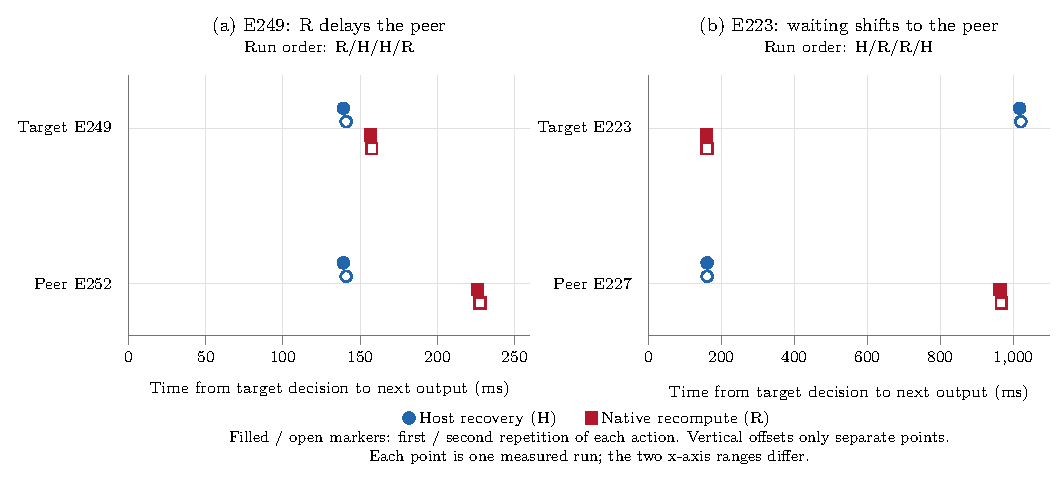
\includegraphics[width=\linewidth]{recovery_next_output.pdf}
\caption{两组单事件干预的原始点，每组每个动作重复两次；均以目标选择时刻为起点，两个面板的横轴尺度不同。目标变快可能伴随邻请求延后；后续输出与工作量不同，此图不是整组加速或自适应策略收益。}
\label{fig:peer-effects}
\end{figure}

\section{独立 MultiNews 六臂：零恢复覆盖与质量限制}
\label{sec:multinews}
\code{oct07_multinews_r01} 已按 H/R/L/L/R/H 完成六臂，每臂 256 请求，新增 1536 次执行。冻结输入来自官方 LongBench MultiNews~\cite{longbench}：27 个完整新闻组按固定次序重复为 192 个长请求，配合原 64 条短题。长请求 prompt 为 2534--3040 tokens，输出 cap 为 1024；参考摘要只用于离线评分。L 在共同合法域内以当前已知历史 $n\le1792$ 选原生重算，否则 Host。1792 来自固定量子 2048 减配置上限 256 个单 token decoder，是预声明的静态基线，不保证其他 prefill 存在时仍有这份预算；未据本组时延调参。

六臂均完整结束，每臂输出 82,929 tokens，抢占、恢复决策、提交、共同合法事件、fallback 与 LOAD 均为零。因此 H/R/L 没有实际动作分叉，也未覆盖长度规则的短侧。全部 15 对逐请求完整 token 序列和完成/停止元数据一致；显式映射内部 ID 后，保留批内顺序的 1197 步调度、计算位置及分配后空闲块也完全一致。逐步运行/等待数与 Host 常驻状态同样一致。

\begin{table}[htbp]
\centering\small
\caption{MultiNews 正式服务；六臂均无恢复且工作相同，时延差异不能归为名义策略收益。}
\label{tab:multinews}
\begin{tabular}{@{}lrrrrr@{}}
\toprule
臂 & 完工(s) & 平均完成(s) & P95 完成(s) & P99 间隔(ms) & 最大间隔(ms) \\
\midrule
H0 & 40.811 & 22.904 & 36.293 & 73.872 & 99.826 \\
R1 & 41.172 & 23.119 & 36.614 & 74.270 & 112.833 \\
L2 & 41.158 & 23.204 & 36.723 & 76.317 & 106.452 \\
L3 & 41.056 & 23.120 & 36.602 & 73.952 & 108.903 \\
R4 & 41.137 & 23.182 & 36.660 & 75.739 & 114.855 \\
H5 & 41.189 & 23.146 & 36.632 & 76.269 & 118.582 \\
\bottomrule
\end{tabular}
\end{table}

完工时间跨度 0.378305 s（相对最短值 0.927\%）是本次相同执行的波动。每臂原生实际调度 661,423 个位置，等于输入 578,750 加实际输出 82,929 减请求数 256；重复历史位置为零。输出 cap 总和 212,992 不是实际工作量。每臂实际 STORE 为 80.5625 GiB、5742 个报告传输，各臂 CUDA-event 时间和介于 1.688484--1.706157 s；LOAD 字节与时间为零。全部 STORE 成本保留，事件时间和不能与计算相加为墙钟，预热不混入正式结果。

六臂在 step 298 分配后均达到观测峰值 32,235/36,916 blocks，即 87.319861\%（含初始非空闲的一块），Host 常驻峰值为 32 GiB。该时点前已有 64 请求自然退出，剩余 192 个；同一步两个请求完成释放的 $55+47=102$ blocks 与空闲块增长相符。这是实际调度与完成释放证据，不是输出 cap 推算。仅用步末采样会漏掉 90 blocks 的峰值，当前口径也不宣称完整 allocator 高水位。Host 满不意味着存在可恢复请求；本组没有被抢占请求或合法候选。原始复核见\code{multinews_results.txt}。

\paragraph{官方重叠评分与人工忠实性边界。}
冻结评分器的输入、身份、自然停止配置及完整输出检查通过。按官方 LongBench ROUGE-L F1 行为，对每条输出取官方参考中的最高分，再先在重复请求内平均、后对 27 新闻组等权平均，六臂均为 27.242567（0--100）；192 请求加权均值为 27.247285。长请求实际输出均值 398.656 tokens，188 条 stop、4 条 length，空输出、评分异常及生成错误记录均为零；length 仍在分母。所有 15 对总体及逐新闻组分数相同，不能将 192 次重复或六臂视作更多独立文档。

预先固定的三个身份只各审阅一份跨臂相同文本。E001 将仍在留守写成晚间已遵令离开的含义，并混淆城市处置；E035 将原文七岁的妹妹写作九岁的 ``Sarah''，姓名未由输入提供。E018 的主要事实受到输入支持，但有覆盖省略。三条均无明显循环复读或可见截断，这不抵消事实问题；该样本也不能估计整体错误率。官方参考本身有输入未支持的细节及来源间差异，故保留冻结 gold，同时以完整输入核验忠实性。ROUGE、自然 stop 或评分无异常均不认证摘要质量通过。本组的输出一致性不能验证未发生的恢复状态连续性。证据见\code{multinews_quality.txt} 与\code{multinews_quality.json}。

\section{已完成的预算规则八臂：等价性与淘汰}
\label{sec:budget-next}
本组测试的规则 B 只在现有 Host 就绪与完整历史容量检查确认两路径共同合法时读取当前原生 schedule 的剩余 token 预算 $q_t$：
\begin{equation}
 \pi_B(n_r(t),q_t)=
 \begin{cases}\mathrm{Recompute},&n_r(t)\le q_t,\\
 \mathrm{Host},&n_r(t)>q_t.
 \end{cases}
\end{equation}
域外沿用相同原生 fallback。$q_t$ 是尚可调度的精确 token 数，不是 GPU 时间或成本预测；规则没有拟合阈值，不读取未来输出，也不预执行两分支。它检验本步原生计算余量是否比固定 1792 长度条件更有用，不预设较短重算会减少服务步数或改善完整服务。

薄观测层包裹原生 schedule 和分配调用，不复制调度器；从原生每步 token 上限开始，仅成功的正 token 分配扣减预算，失败分配及零 token 异步 LOAD 不扣减。每步结束按请求 ID 及总量与原生\code{SchedulerOutput.num_scheduled_tokens} 精确核对，不支持的配置或不一致均显式失败。该实现限定现有 FCFS、同步、无推测等已支持配置，所有固定方式、L/B 及共同预热使用相同观测层，不改变调度或传输机制。

\paragraph{真实执行与观测完整性。}
\code{oct07_budget_r01} 已按冻结顺序 H/R/L/B/B/L/R/H 完成八臂，每臂 256 请求，新增 2048 次执行；同组复用原自然长摘要输入、正常 0.9 profiling 得到的 72.1015625 GiB GPU KV、32 GiB pinned Host 及相同完整预热。L 的阈值仍为预声明的 1792，没有据本组重新拟合。八个正式 episode 与八次预热共 33,010 条预算观测全部为\code{CHECKED}，错误为零；每步运行时的逐请求分配核验、离线原生调度总量及余额、decision/commit 关联与时间包含检查均通过。正式步数依次为 1993、2016、2024、2024、2024、2024、2016、1993，八次预热各 2112 步。本组没有额外 drain 调度步，服务后排空时间仍保留。33,010 是观测完整性检查数，不是独立性能试验数。

全组新增 74 次共同合法提交，其中 52 次 Host、22 次重算；它们也不是 74 个独立干预。H 两臂各有 14 次共同合法 Host 与 22 次 Host-miss 原生重算 fallback；R 两臂各有 9 次共同合法重算与 27 次相同类型 fallback。四个 L/B 臂各有 7 次合法选择（6 Host、1 重算）及 28 次 Host-miss fallback。所有合法提交的请求状态保留检查通过，恢复到下一输出的匹配无 censor；该检查仍不替代 KV、logits 或随机采样正确性验证。

\paragraph{B 与固定阈值完全等价的观测域。}
在本组全部 74 个合法 decision/commit 上，以当时已知历史和剩余预算重放 B 与 L1792，动作分歧为零。尤其四个 L/B 臂的合法序列完全一致：$(n,q,a)$ 依次为 $(2736,1845,H)$、$(706,1852,R)$、$(3128,1856,H)$、$(3222,1882,H)$、$(3226,1883,H)$、$(3234,1884,H)$、$(3515,1884,H)$。预算仅在 1845--1884 变化，合法前缀在 706 与 2736 之间没有样本，因此任意 706--2735 的整数长度阈值都可重现这四臂的动作。这个区间只是事后等价性诊断，未被重新选作策略阈值，也不构成跨臂反事实结果。

显式映射内部 ID 后，保留每步请求顺序、调度 token 数、计算起止位置及已知/已生成进度的 2024 步原生轨迹，在四个 L/B 臂中完全相同；规范化 SHA256 为\code{fdf4b73363c38a4c9bf79ee7aa8df7dae4cafe24bb631a3a21db390747885625}。它们全部 256 条逐 token 输出也一致。B 并未退化成单一固定动作，而是在当前实际可恢复域内与固定长度阈值没有差别；不能将跨臂小幅计时波动归为状态选择收益。

\begin{table}[htbp]
\centering\small
\caption{预算八臂正式服务。下一输出列为各臂共同合法提交均值；H/R/L 的合法事件域不同，不能直接配对这些局部均值。}
\label{tab:budget-results}
\begin{tabular}{@{}lrrrrr@{}}
\toprule
臂 & 完工(s) & 平均完成(s) & P99 间隔(ms) & 下一输出(ms) & 实际输出 \\
\midrule
H0 & 88.244 & 57.033 & 82.615 & 310.405 & 189,436 \\
R1 & 89.455 & 57.900 & 82.250 & 158.448 & 191,080 \\
L2 & 89.281 & 57.623 & 83.234 & 153.893 & 189,035 \\
B3 & 89.369 & 57.693 & 83.678 & 153.813 & 189,035 \\
B4 & 89.414 & 57.728 & 83.683 & 154.003 & 189,035 \\
L5 & 89.675 & 57.916 & 85.341 & 154.513 & 189,035 \\
R6 & 91.072 & 59.023 & 87.098 & 159.063 & 191,080 \\
H7 & 89.577 & 57.866 & 83.304 & 314.198 & 189,436 \\
\bottomrule
\end{tabular}
\end{table}

前序 L2/B3 中 B 慢 0.088194 s，反序 B4/L5 中 B 快 0.260532 s；B/L 完工均值分别为 89.391496/89.477665 s，相差约 0.096\%。由于两者动作、原生轨迹和输出完全相同，这个微小差异不构成自适应收益。每种策略只有两次运行，不能把各次抢占和检查数扩大为独立重复。

\paragraph{完整工作与质量边界。}
H/R/L/B 每臂实际调度分别为 860,683/894,640/876,883/876,883 个 token 位置，重复已知历史分别为 72,886/105,199/89,487/89,487。同策略两次工作量一致。每个 H/R/L/B 臂 STORE 字节依次为 103,551,074,304、103,309,901,824、103,083,409,408、103,083,409,408；LOAD 字节为 4,349,493,248、0、1,983,905,792、1,983,905,792。L/B 每臂为 6 次 LOAD、12,390 次 STORE；B 两臂每臂报告的 STORE CUDA 时间约 2.082 s，LOAD 约 0.0359 s。历史 STORE 全部保留，传输可与计算重叠，不能相加为墙钟。观测最低的固定 H 完工均值也不能直接称为等输出工作加速，因为 H/R/L 的自然输出量及后续内容不同；H 与 L/B 有 193/256 条输出不同，H 与 R 有 197/256 条不同。

另按已有冻结规则独立评分本组 64 条短题，八臂均为 26/64（40.625\%）；H/L/B 各一条 length，R 各三条 length。\code{budget_short_quality.json} 保留逐请求数值、停止类型及原始 token 绑定。这只是限定数值与自然停止指标；同分不能证明质量等价，也不认证长摘要忠实性。原始指标和规范化轨迹证据见\code{budget_results.txt}、\code{execution/oct07_budget_r01/budget_summary.json}及\code{execution/oct07_budget_r01/budget_trace_consistency.json}。现有局部\code{adapter_seconds} 不含整个预算观测层；包住原生 schedule 的 span 包含调度本身，完整插桩开销尚未分离。

\paragraph{淘汰而非继续拟合。}
本组完成了真实 GPU 验证，也否定了当前恢复域内预算信号的实际增量动作价值。活动执行路径已撤下 B 及其预算 observer，H/R/L 的原生执行保持不变。新的容量余量规则随后完成下文六臂核验，仍未建立全服务收益。八臂原始数据与分析保存在\code{execution/oct07_budget_r01/}，完整预算代码及 22 项 CPU 测试保存在\code{execution/source_snapshots/oct07_budget_r01/}，以复现本次负结果。该结论只限定当前信号和观测域，不能推出所有状态选择均无效；不继续搜索预算参数，也不改变固定调度机制来制造动作分歧。

\section{短重算的连续服务反例}
\label{sec:short-repreempt}
四个 L/B 臂唯一一次共同合法重算均为 E252/event37/step357，与先前冻结的短恢复身份完全匹配：已知 706 tokens，其中已生成 35、prompt 671，正 Host 命中 656；完整状态需要 45 blocks，当时 free52、reserved0。H0/H7 与 L2/B3/B4/L5 在 step0--356 的全部已生成历史、规范化调度、逐步输出以及此前恢复和抢占记录，15 对比较全部一致。原短事件 spec 未作为本组在线 one-event 条件执行；这是全策略运行内的事后机制诊断，不能改称另一次冻结单点试验。

\begin{table}[htbp]
\centering\small
\caption{同一 E252 短恢复的首次进展与后续停顿；六臂该请求最终均为相同 56 tokens、自然 stop。}
\label{tab:short-repreempt}
\begin{tabular}{@{}lrrr@{}}
\toprule
臂 & 选择到下一输出(ms) & 随后的生成间隔(s) & 请求完成(s)\\
\midrule
H0 & 276.438 & 0.069660 & 63.052265\\
L2 & 72.293 & 45.491467 & 67.306284\\
B3 & 72.403 & 45.496164 & 67.336100\\
B4 & 72.213 & 45.607057 & 67.446346\\
L5 & 72.280 & 45.748773 & 67.642654\\
H7 & 278.589 & 0.070206 & 64.012691\\
\bottomrule
\end{tabular}
\end{table}

在 step357，Host 为 E252 加载 41 blocks、留下 11 个空闲块；重算完整 706 位置使用 45 blocks、留下 7 块，并立即产生相同的下一 token878。两种方式都让同一批 196 个其他请求完成一个 decode，故不能说此次短重算挤掉了当步其他 decode 机会。Host 的 82 MiB LOAD 在该步末已经完成，CUDA-event 仅约 1.57 ms，但必要尾部直到 step360 才获得计算机会。重算臂却在紧接的 step358、free0 时再次抢占 E252；刚恢复的 706 个计算位置没有保证它继续驻留。其下一个 token281 要等 step994 的 Host-miss 原生重算，形成表中的约 45.5 s 停顿。

机会同时发生交换：E250 在 L/B 中先得到 step359--361 三次 decode，再于 362 被抢占；H 中它在 359 就被抢占。E250 随后也有长等待，不能把两个请求的等待加减成墙钟收益。H 中 E252 之后仍会再次抢占，其最大生成间隔本身约 40.85--41.53 s；Host 也不是无停顿服务。对同一个最终 56-token 输出，E252 的累计调度位置由 H 的 1510 增为 L/B 的 2137，重复历史多 627 位置。全组后续轨迹和其他输出仍会改变，不能把所有全局差值都归给这 627 个位置。

这个反例直接区分了“下一次输出提前”和“持续恢复成功”。共同完整状态容量检查确认当前动作可行，却没有保证下一轮容量或 victim 地位；剩余计算 token 预算也不包含这个风险。原始逐步证据与全部重复见\code{budget_short_event_diagnostic.txt}。下节实际检验决策前可见的 KV 余量能否解释这一具体机制，不据此预设在线收益。

\section{容量余量规则与六臂真实验证}
\label{sec:multinews320-next}

\paragraph{先验证一个有具体机制的容量信号。}
令当前完整恢复后的空闲余量为 $s_t=B_{\mathrm{free}}-B_r-B_{\mathrm{reserved}}-B_{\mathrm{watermark}}$。在当前全部 running 都满足已知长度 $n_i=c_i+1$、非 prefill chunk 且没有原生跳过条件时，读取
\begin{equation}
 m_t=s_t-\sum_{i\in\mathrm{running}}\mathbf1[n_i\bmod b=0]
           -\mathbf1[n_r(t)\bmod b=0].
\end{equation}
原生 computed 计数在整步调度结束时才增加；在已核验的同步单卡 FCFS 路径上，waiting lookup 此时已知这些 running 请求成功获得当步一个 token 的分配。式中计数是该集合若继续生成一 token 的下一轮新增块数，不读取未来 EOS 或输出长度。G 仅在原共同合法域、$n_r\le1792$、背景支持且 $m_t\ge0$ 时重算；其余选 Host。背景不支持时记录空 margin 和独立 policy reason，仍保留共同合法标记，不把原生重算说成不可执行。

冻结前 H 轨迹的两个 E252 点分别给出 $52-45-0-10=-3$ 与 $91-45-5-10=31$ blocks；当时后一状态还没有真实重算对照。这支持一次有界验证。新规则只添加该容量信号，通过 15 项 CPU 检查及独立源码审计后，已按 H/L/G/G/L/H 完成串行 GPU 对照。各臂等量记录支持域及余量，原生分配器、victim、队列、量子和传输不改。lookup 后的新准入、集合外异步尾部及后续完成均可改变容量，因此正 margin 不是下一步免抢占保证。实现与适用域见\code{headroom_selector_note.txt}、\code{headroom_signal_audit.txt}和\code{headroom_next.txt}。

\paragraph{状态、动作与连续性通过实测核验。}
\code{oct07_headroom_r01} 六臂新增 1536 次正式执行，60 次共同合法 lookup 均成功提交，其中 56 Host、4 重算。各臂的请求身份、已知历史和输出前缀连续性检查通过。60 次提交中 54 次处于支持域，6 次背景不满足单 token 就绪条件，全部出现在两个 H 臂；其 margin 为 null，未误记为原生重算不可行。两个 G 臂各有 9 次共同合法提交，全部处于支持域，实际为 8 Host 加 1 重算。离线分析通过 10,558 条背景请求与原生单 token 分配的一致性检查；该数不是独立性能样本数，也不是 KV 或 logits 数值等价证明。

G 在 E252 已知 706 tokens、margin $=-3$ 时保留 Host，在已知 719 tokens、margin $=31$ 时选择重算。这不是 $n\le\tau$ 选重算的单调长度规则可同时产生的动作组合；但二者的前缀、Host 命中覆盖及历史也不同，不能据此排除所有静态成本解释。所有六臂在首次分歧前保持完整历史和调度一致；H/G 四臂在第二个分歧前亦一致。此处是全策略运行中的轨迹核验，没有事后重命名为新增的单事件随机化实验。

\begin{table}[htbp]
\centering\small
\caption{容量余量六臂的实际完整服务。存在同策略计时漂移和跨策略输出差异，不能解释为等工作量加速。}
\begin{tabular}{lrrrrr}
\toprule
臂 & 完工 (s) & 平均完成 (s) & P99 间隔 (ms) & 最大间隔 (s) & 输出 tokens\\
\midrule
H0 & 97.710 & 63.222 & 98.196 & 51.855 & 189,436\\
L1 & 106.434 & 64.547 & 94.358 & 53.085 & 189,035\\
G2 & 100.456 & 64.066 & 113.533 & 53.261 & 190,178\\
G3 & 114.256 & 65.269 & 98.733 & 50.791 & 190,178\\
L4 & 98.939 & 64.722 & 107.494 & 57.130 & 189,035\\
H5 & 111.679 & 63.615 & 99.398 & 46.591 & 189,436\\
\bottomrule
\end{tabular}
\end{table}

\paragraph{局部持续进展改善，代价仍转移给其他请求。}
六臂 E252 最终均为相同的 56-token 自然停止输出。L 在 706 处重算后仍立即再次抢占，随后生成间隔为 50.340/54.816 s。G 在该点用 Host，随后在 719 处重算，到下一输出为 72.657/84.210 ms，紧接间隔为 70.194/84.733 ms，最终完成为 22.409/26.771 s，最大生成间隔仅 0.489/0.578 s。对应 H 的完成为 69.758/68.111 s，最大生成间隔为 47.613/42.057 s；L 的完成为 75.474/76.884 s。这建立了实际目标请求的持续进展改善，不只是提前一个 token。

然而 G 消除 E252 在 step382 的第三次抢占后，原生 victim 变为 E249；H 中 E249 到 step386 才被抢占。G 中 E252 比 E249 提前一轮加入 running，改变了原规则选择的尾部 victim。E249 的相同内容输出 \#79，在 H 的 step382 产生，在 G 延至 step972；以 719 决策为起点，等待由 H 的 365--382 ms 变为 G 的 46.23--49.15 s。H 后来也会抢占 E249，因此不能把两者等待简单相加减为墙钟。全局 G 完工均值为 107.356 s，H 为 104.694 s，G 与 L 的完工排名在正反序块中翻转。完整逐步诊断见\code{headroom_event_diagnostic.txt}。

\paragraph{实际工作、开销与质量限制。}
每个 H/L/G 臂分别调度 860,683/876,883/870,682 个 token 位置，重复已知历史 72,886/89,487/82,143 个；G 相对 H 的新增 9,999 个位置中有 742 个是新增输出，其余 9,257 个为重复历史。STORE 字节分别为 103,551,074,304、103,083,409,408、103,219,724,288；LOAD 字节分别为 4,349,493,248、1,983,905,792、2,508,193,792。H/L/G 每臂另有 22/28/25 次 Host-miss 原生重算 fallback。全部实际成本保留，不能把后续轨迹的 STORE 差异解释为当前动作避免了已付成本，也不能相加 CUDA 时长得到墙钟。

每个策略内部两次运行的全部输出及停止元数据一致，H/L 跨策略有 193 条输出不同，H/G 与 L/G 各有 196 条不同。H、L、G 同策略两次完工差分别为 13.969、7.494、13.800 s；这些差异必须保留，不用离线校正构造收益。已测 adapter span 每臂合计 17.4--31.2 ms，尚不包含其他 hook、输出日志与完整 observer 开销，因此完整开销控制仍未完成。

独立计时复核确认 H、L、G 重复内的全部 1993、2024、2005 步规范化原生轨迹一致；差异主要集中在最多 32 个请求的步骤及终末阶段。H5--H0 的 step 墙钟与 driver 线程 CPU 差为 14.357/14.363 s，G3--G2 为 14.500/14.516 s。计算阶段 626 条有效 GPU 采样未见额外计算 PID，慢尾段的 SM/显存时钟仍为 2422/12481 MHz，GPU 利用率和功率更低；温度方向不支持已证实的热降频解释。线程 CPU 可包含驱动忙轮询，不能视为纯主机计算，也不能用墙钟减 CPU 得到 GPU 时间。具体根因尚未隔离；下节已完成的固定 Host 旁观测开关干预未消除漂移。详见\code{headroom_timing_diagnostic.txt}。

冻结的短题评分六臂均为 26/64，各有一条 length、零条无法解析。G 相对 H/L 有四条短题输出不同，正确题集合虽未变，却不证明输出或总体质量等价；本组未新增长摘要事实性认证。指标、源代码哈希和原始结果见\code{headroom_results.txt}、\code{headroom_summary.json}及\code{headroom_short_quality.json}。最小状态规则已可执行且有增量动作信息，但目前仍只是实验候选，不能称为全服务最优策略。

\section{GPU 旁观测开关的真实对照}
\code{oct07_telemetry_r01} 按固定 H 的 ON/OFF/OFF/ON 完成四臂；只切换冻结旧版 1 Hz GPU 查询子进程，逐步 CPU 计时、请求输出和原生轨迹记录不变。1024 个到达请求全部完成，无失败、拒绝、超时或未完成。每臂 14 次共同合法提交均为 Host，另有 22 次 Host-miss 原生重算 fallback。恢复方式差异为零，不能把这一测量干预写成选择器收益。

六个配对的 256 条完整输出和停止元数据、1993 步规范化原生调度完全一致。每臂实际输出 189436 tokens，调度 860683 位置，其中重复 72886。正常容量、输入与外到达、预热和原生引擎配置相同；逐臂身份验证通过。
\begin{table}[htbp]
\centering\small
\caption{相同工作量的 GPU 遥测开关对照。尾段预定义为最后一次超过 32 个调度请求后的步骤；每臂为 731 步、9026 个位置。}
\begin{tabular}{lrrrrr}
\toprule
臂 & 查询 & 完工 (s) & 完成均值 (s) & TTFT 均值 (s) & 尾段 (s)\\
\midrule
H0 & ON  & 99.973 & 63.006 & 7.803 & 12.994\\
H1 & OFF & 107.917 & 64.673 & 8.294 & 21.161\\
H2 & OFF & 101.938 & 64.068 & 7.816 & 13.348\\
H3 & ON  & 103.314 & 63.885 & 7.953 & 17.215\\
\bottomrule
\end{tabular}
\end{table}

正序关闭查询后尾段慢 8.168 s，反序关闭后快 3.867 s；两个 OFF 尾段仍相差 7.813 s。2--8 个请求桶的步耗时中位数为 12.624/34.556/12.623/32.802 ms，快慢均可出现在 ON 或 OFF。driver CPU 时间与增加的墙钟近乎同步，不能由此区分主机执行和 CUDA 忙轮询。ON 两臂共 204 个正常样本，采样与四臂端点未发现其他 GPU 计算 PID；这一检查不能覆盖采样间隔或 OFF 全程。本组不支持把旧 GPU 查询定为漂移根因，也不证明它零开销；不追加重复或扫描频率。

每臂已付 STORE 为 103551074304 bytes、LOAD 为 4349493248 bytes；不从服务时间扣除旁观测或传输事件时间。四臂最大生成间隔依次为 50.622/51.301/51.599/51.521 s。逐请求完成、生成间隔、发送滞后和完整成本保存在\code{telemetry_results.json}及原始组的\code{telemetry_control_summary.json}中；分析命令为\texttt{python3}\enspace\code{analyze_telemetry_control.py}\enspace\code{execution/oct07_telemetry_r01}。只有整组结束、进程退出及共享 GPU 锁释放后才回读归档。

下一项限定诊断为两个固定 H 重复，加入被动的主线程 CPU 当前频率、上下文切换及容器 CPU 限流快照。已完成 CPU-only 可用性预检，并冻结\code{cpu_tail_control.json}；GPU 诊断尚在候锁，不计入上述结果。该观测不改变策略、进程亲和性、频率或优先级。若慢段伴随这些读数变化，才能据此设计一次具体控制；若不复现或信号无区分力，不自动重复、调参或声称消除了计时问题。相关性不作为因果证明，也不生成校正时延。

\section{后续独立新闻容量域验证}
\paragraph{已冻结的输入候选。}
MultiNews256 已完成组的实测 GPU KV 观测峰值为 87.319861\%，六臂均无恢复，尚未覆盖该独立任务的容量竞争域。一个已在 CPU 冻结、GPU 尚未运行的后继候选为 320 请求组，状态为\code{CPU_FROZEN_GPU_UNRUN}，尚未排队。H/R/L/G/G/L/R/H 的后继设计和分析接口已准备，L1792 与 G 的容量门均不变，但先处理同工作计时漂移，不立即扩展八臂矩阵。输入保留原 64 条短题和 192 条完整新闻请求，再沿冻结的同一来源次序追加 64 条长请求，成为 64 短加 256 长。仍只有 27 个新闻组被重复提交，不能称为 320 个独立文档样本。

本候选统一将\code{max_num_seqs}从 256 提到 320，以允许更丰富的同时在途请求；同组八臂必须使用相同设置。模型仍为已有 OLMoE BF16，GPU KV 仍原生 0.9 profiling，Host 32 GiB、每步 2048 tokens、完整当前历史容量检查、自然 EOS 和原有队列/victim/传输机制保持冻结。跨组的并发上限变化必须披露；新引擎需要重新记录实际 KV pool，不能假定其字节数等于旧 256 组。短/长输出上限仍为 256/1024，完整 prompt、参考摘要和评分规则不因本组改写。

冻结输入见\code{inputs_multinews320/pro6000_multinews_candidate_320.json}，设计边界见\code{multinews320_design.txt}与\code{multinews320_headroom_next.txt}。按 prompt 几何计算的假想共同驻留需求只用于说明候选由来，不能作为新组实测峰值、发生抢占或策略获益的证据；也不能将旧组 87.32\% 按请求数线性外推。实际分块 prefill、准入、自然完成释放及重新 profile 的容量都可能使机制仍不触发。若再次零恢复，或只有长恢复使 G 与 H 相同，应保留该适用域边界，不修改到达或限容强迫机制触发，不自动追加参数扫描；尚未执行的 320 组不计入本文四十四格、10752 次执行和 340 次合法提交的累计数。

\clearpage
\begin{thebibliography}{9}
\footnotesize
\setlength{\itemsep}{1pt}
\bibitem{cacheopt} Haiying Shen and Tanmoy Sen. Mitigating KV Cache Competition to Enhance User Experience in LLM Inference. arXiv:2503.13773v1, 2025. \url{https://arxiv.org/html/2503.13773v1}.
\bibitem{stream2llm} Rajveer Bachkaniwala et al. Stream2LLM: Overlap Context Streaming and Prefill for Reduced Time-to-First-Token. arXiv:2604.16395v1, 2026. \url{https://arxiv.org/html/2604.16395v1}. Official artifact: \url{https://github.com/rajveerb/stream2llm/tree/mlsys_artifact}.
\bibitem{unboxkv} Characterizing the Behavior and Impact of KV Caching on Transformer Inferences under Concurrency. Author-hosted full text, 2025. \url{https://jcernuda.com/publications/kv-caching}.
\bibitem{cake} Shuowei Jin et al. Compute Or Load KV Cache? Why not Both? arXiv:2410.03065v2, 2025. \url{https://arxiv.org/html/2410.03065v2}.
\bibitem{cachegen} Yuhan Liu et al. CacheGen: KV Cache Compression and Streaming for Fast Language Model Serving. SIGCOMM 2024; inspected arXiv:2310.07240v4. \url{https://arxiv.org/html/2310.07240v4}.
\bibitem{lumen} Zhang Cao et al. LUMEN: Coordinated Failure Recovery for Distributed LLM Serving. arXiv:2606.17787v1, 2026. \url{https://arxiv.org/html/2606.17787v1}.
\bibitem{shadowserve} Xingyu Xiang et al. ShadowServe: Interference-Free KV Cache Fetching for Distributed Prefix Caching. arXiv:2509.16857v1, 2025. \url{https://arxiv.org/html/2509.16857v1}.
\bibitem{gsm8k} OpenAI. Grade School Math, public test data. Selected test indices 128--191; file hashes preserved in the experiment freeze receipt. \url{https://github.com/openai/grade-school-math/blob/master/grade_school_math/data/test.jsonl}.
\bibitem{longbench} LongBench official data: \code{multifieldqa_en} and \code{multi_news}; revision \code{5e628be450b7e67fb7ae6e201bd6d8f7056f7672}. Evaluation commit \code{2e00731f8d0bff23dc4325161044d0ed8af94c1e}; selected source rows and hashes preserved in freeze receipts. \url{https://huggingface.co/datasets/zai-org/LongBench/tree/5e628be450b7e67fb7ae6e201bd6d8f7056f7672}.
\end{thebibliography}
\end{document}
